% AAAI submission. NOTE: drop in official aaai2026.sty + aaai.bst before final compile.
% Placeholder uses twocolumn article to approximate AAAI layout.
\documentclass[letterpaper,twocolumn,10pt]{article}
\usepackage{times}
\usepackage{amsmath,amssymb,amsthm,booktabs,graphicx,xcolor}
\newtheorem{proposition}{Proposition}
\newtheorem{lemma}{Lemma}
\newtheorem{corollary}{Corollary}
\newtheorem{definition}{Definition}
\usepackage[margin=0.75in]{geometry}
\usepackage{algorithm}
\usepackage{algpseudocode}
\usepackage[numbers]{natbib}
\usepackage{hyperref}

\title{\textbf{Muon Gets Dynamical Isometry for Free:\\ Orthogonalizing Optimizers Preserve Plasticity in Continual Learning}}
\author{Anonymous Submission}
\date{}

\begin{document}
\maketitle

\begin{abstract}
Neural networks trained continually on a stream of tasks progressively lose their ability to learn new ones---\emph{loss of plasticity}. The current state of the art, AdamO (ICML 2026), argues that plasticity is preserved by keeping the network near \emph{dynamical isometry} (layer-wise Jacobian singular values near one, equivalently a well-conditioned empirical NTK), and enforces this with an explicit weight-space isometry regularizer on top of Adam. We make a simple but consequential observation that AdamO did not test: the modern \emph{Muon} optimizer, which orthogonalizes its update at every step, attains dynamical isometry \emph{for free}. Across class-incremental CIFAR-100 (ResNet-18) and permuted-MNIST (MLP), Muon-based continual learning matches or beats AdamO at its best-tuned regularization strength, and under a fully matched comparison---both methods given the same unit-reperturbation and tuned hyperparameters---Muon beats AdamO by $+9.3$ points ($t{=}8.4$, $n{=}5$) on CIFAR-100. The mechanism is direct: Muon maintains a penultimate-layer effective rank of ${\sim}167$ over the task stream \emph{without any regularization}, well above the ${\sim}107$ that AdamO reaches even at its \emph{best-tuned} isometry penalty, and far above Adam's ${\sim}59$. We confirm with a $2{\times}2$ optimizer$\times$reperturbation decomposition that the orthogonalizing base---not the reperturbation---carries the gain, and we are explicit about scope: plain Muon underperforms a strongly-regularized AdamO on deep residual networks unless paired with reperturbation, and a competing optimizer-state re-conditioning lever helps only on MLPs. Our results reposition the optimizer, rather than an added regularizer, as the primary lever for plasticity.
\end{abstract}

\section{Introduction}
A central obstacle to lifelong learning is \emph{loss of plasticity}: as a network is trained on a stream of tasks, its capacity to fit \emph{new} tasks deteriorates, even when retaining old tasks is not the concern~\citep{dohare2024}. This is the failure mode that prevents a single network from being trained indefinitely on a non-stationary data stream, and it is distinct from catastrophic forgetting---it concerns the acquisition of \emph{new} knowledge rather than the retention of old. Strikingly, the workhorse optimizer of deep learning, Adam, \emph{accelerates} the decline relative to plain SGD~\citep{dohare2024}. The phenomenon has been traced to representational pathologies---dormant and dead units~\citep{sokar2023}, effective-rank collapse, and Hessian spectral collapse~\citep{spectralcollapse2025}---and to weight-space drift away from well-conditioned regions of parameter space~\citep{kumar2023}. A common thread runs through these diagnoses: as training proceeds the network's representations and gradients concentrate into an ever-smaller subspace, and the optimization dynamics become progressively ill-conditioned.

The current strongest single method, \textbf{AdamO}~\citep{adamo2026}, gives this a clean theoretical frame. It defines plasticity functionally through the empirical Neural Tangent Kernel (NTK) and argues that task-agnostic plasticity is governed by the \emph{anisotropy} (condition number) of the NTK: a well-conditioned, near-isotropic NTK lets gradient descent make comparable progress in all output directions. The tractable surrogate is \emph{dynamical isometry}---keeping every layer's input--output Jacobian singular values near one. AdamO enforces this with a decoupled Gram-deviation penalty $\|W^\top W - I\|_F^2$ added to Adam, driving \emph{all} singular values toward one, and reports state-of-the-art plasticity across supervised and RL continual benchmarks.

\textbf{Our observation.} AdamO works hard---via an explicit, tuned regularizer---to keep the optimization dynamics well-conditioned. But there already exists an optimizer whose update is \emph{constructed} to be well-conditioned: \textbf{Muon}~\citep{muon2024}, which orthogonalizes its momentum via a Newton--Schulz iteration before each step, so that the update direction has near-uniform singular values by design. AdamO never tested the Muon \emph{optimizer} (its ``NS'' baseline is a periodic weight-projection, not Muon). We ask: does an orthogonalizing optimizer obtain the dynamical isometry that AdamO regularizes toward---\emph{for free}---and does that translate into better plasticity?

We find that it does. Our contributions:
\begin{enumerate}\itemsep2pt
\item We show the modern Muon optimizer is a strong continual-learning base: it maintains a penultimate effective rank ($\sim$167) well above the best-regularized AdamO ($\sim$107) and roughly \emph{three times} that of Adam ($\sim$59), with no plasticity-specific regularization (\S\ref{sec:mech}).
\item Under a fully matched, best-hyperparameter comparison on class-incremental CIFAR-100, Muon (with unit reperturbation) beats AdamO (with the same reperturbation) by $+9.3$ ($t{=}8.4$, $n{=}5$); the advantage holds, more modestly, on permuted-MNIST (\S\ref{sec:exp}).
\item A $2{\times}2$ optimizer$\times$reperturbation decomposition isolates the \emph{orthogonalizing optimizer} as the source of the gain---CBP-style reperturbation on Adam reaches only $51.6$ versus Muon's $78.2$ (\S\ref{sec:exp}).
\item We are explicit about scope (\S\ref{sec:scope}): plain Muon loses to a strongly-regularized AdamO on deep ResNets unless paired with reperturbation; an optimizer-state re-conditioning lever helps on MLPs but not ResNets; and Muon's apparent ``collapse'' at high learning rate is a tuning artifact, not a plasticity failure.
\end{enumerate}

\section{Related Work}
\textbf{Loss of plasticity and its diagnostics.} \citet{dohare2024} establish the phenomenon at scale across supervised and reinforcement learning and propose Continual Backprop (CBP), which continually reinitializes the least-useful units. A diagnostic literature attributes the loss to specific pathologies: dormant and dead ReLU units~\citep{sokar2023}, collapse of the representation's effective rank, and collapse of the Hessian/NTK spectrum~\citep{spectralcollapse2025}. These diagnostics motivate \emph{effective rank} as the quantity we track. \textbf{Representation resets.} CBP~\citep{dohare2024} and ReDo~\citep{sokar2023} reinitialize low-utility or dormant units; shrink-and-perturb~\citep{ash2020} perturbs all weights each task. These act on the representation and are agnostic to the optimizer. \textbf{Weight-space regularization.} L2-init / regenerative regularization~\citep{kumar2023} pulls weights toward their initial values; AdamO~\citep{adamo2026} adds a decoupled dynamical-isometry (Gram-deviation) penalty $\|W^\top W-I\|_F^2$ and is, to our knowledge, the strongest published single method. A central claim of AdamO is unifying: it reinterprets prior heuristics (Normalize-and-Project, spectral-norm regularization, weight decay) as each controlling only a \emph{partial} measure of isometry (the mean or the maximal singular value), whereas its penalty drives \emph{all} singular values toward one. \textbf{Orthogonalizing optimizers.} Muon~\citep{muon2024} orthogonalizes the momentum of each hidden weight matrix via a Newton--Schulz iteration and has become a leading optimizer for standard (single-task) training of transformers and vision models, where its well-conditioned updates accelerate convergence. Its behavior under sustained continual non-stationarity, however, is unstudied---and, crucially, AdamO's ``NS'' baseline is a periodic projection of the \emph{weights} onto the orthogonal manifold, not the Muon \emph{optimizer}, which orthogonalizes the \emph{update} every step. \textbf{Our distinction.} All prior plasticity methods either reset the representation or regularize the weights, leaving the optimizer fixed at Adam. We show that the choice of optimizer is itself a primary lever: an orthogonalizing optimizer achieves better-conditioned dynamics---and higher effective rank---intrinsically, beating AdamO on the very NTK-conditioning terms AdamO is built to optimize.

\section{Background}
\paragraph{Plasticity and the NTK.} Following \citet{adamo2026}, first-order progress on a new task is governed by the empirical NTK $K_\theta(X)=J_\theta(X)J_\theta(X)^\top$, where $J_\theta$ is the parameter--output Jacobian. To first order, a gradient step reduces the loss along output direction $g$ in proportion to the Rayleigh quotient $g^\top K_\theta g/\|g\|^2$; an anisotropic (ill-conditioned) $K$ therefore forces the global learning rate to respect its largest eigenvalue while progress along small-eigenvalue directions stalls, and directions in the nullspace of $K$ cannot be updated at all. Task-agnostic plasticity is thus controlled by the \emph{condition number} of $K$, and the tractable architectural surrogate for keeping $K$ well-conditioned is \emph{dynamical isometry}---keeping every layer's input--output Jacobian singular values near one.

\paragraph{Effective rank.} As our empirical proxy for this conditioning we use the penultimate-layer \emph{effective rank}, $\mathrm{erank}(f_\theta)=\exp\!\big(-\sum_i \tilde s_i\log \tilde s_i\big)$, the exponentiated spectral entropy of the centered post-activation singular values $\tilde s_i$ (normalized to sum to one). It is a standard plasticity diagnostic: a representation that has collapsed onto a low-dimensional subspace has low effective rank, leaving few directions in which a new task can be fit, and it lower-bounds the conditioning of the feature covariance feeding the output head.

\paragraph{Muon.} Muon maintains momentum $m_t=\beta m_{t-1}+g_t$ and applies, for each 2D weight (convolutions reshaped to $[\text{out},\,\text{in}\cdot k^2]$), the orthogonalized update $\theta\!\leftarrow\!\theta-\eta\,\mathrm{NS}(m_t)$, where $\mathrm{NS}(\cdot)$ is a quintic Newton--Schulz iteration approximating $UV^\top$ of the momentum's SVD. The update therefore has near-uniform singular values \emph{by construction}---the very property AdamO regularizes toward.

\section{Method}\label{sec:method}
Our prescription is deliberately minimal: \emph{use an orthogonalizing optimizer as the continual-learning base, optionally paired with unit reperturbation}. We do not add any plasticity-specific regularizer. Concretely (Alg.~\ref{alg:muon}), within each task we train with Muon: convolutional kernels are reshaped to 2D, their momentum is orthogonalized by a five-step Newton--Schulz iteration, and BatchNorm/bias parameters fall back to momentum SGD. The only continual-learning--specific operation is an optional reperturbation (RP) at each task boundary---reinitializing the incoming weights of the lowest-utility units in proportion to a measured effective-rank deficit, a curvature-gated variant of Continual Backprop~\citep{dohare2024}. RP is applied \emph{identically} to whichever optimizer it is paired with, so all comparisons that include it are matched. Crucially, the orthogonalization is what carries the effect; RP is a small, optional booster (\S\ref{sec:exp}).

\begin{algorithm}[t]
\caption{Muon base for continual plasticity (one task)}\label{alg:muon}
\begin{algorithmic}[1]
\State \textbf{at task boundary (optional RP):} $d\!\leftarrow\!\max(0,(r^\star-\mathrm{erank}(f_\theta))/r^\star)$; reinit incoming weights of the lowest-utility $\rho d$ fraction of units
\For{each minibatch}
  \State $g\leftarrow\nabla_\theta\mathcal{L}$;\quad $m\leftarrow\beta m+g$
  \For{each 2D weight $W$ (conv reshaped to $[\text{out},\text{in}\cdot k^2]$)}
    \State $W\leftarrow W-\eta\,\mathrm{NS}_5(m_W)$ \Comment{orthogonalized, full-rank update}
  \EndFor
  \State other params (BN, bias): $W\leftarrow W-\eta\,m_W$
\EndFor
\end{algorithmic}
\end{algorithm}

\section{Experiments}\label{sec:exp}
\paragraph{Setup.} We use three standard plasticity benchmarks spanning architectures and task structures. \textbf{Class-incremental CIFAR-100}: a CIFAR-adapted ResNet-18 (width 32, BatchNorm, residual connections), 25 tasks of 10 random classes each (relabeled $0\!-\!9$), 5000 images, 2 epochs/task. \textbf{Class-incremental CIFAR-10}: the same ResNet-18 on random binary partitions of the ten classes, 40 tasks. \textbf{Permuted-MNIST}: a depth-4 width-512 MLP (matching AdamO's reported architecture), each task a fixed random pixel permutation, 80 tasks, base lr $10^{-4}$. Following the plasticity literature we measure \emph{plasticity} as late-task online accuracy---the mean training accuracy over the final 10 tasks, i.e.\ how well the network still fits \emph{new} tasks after a long stream---averaged over seeds ($n{=}5$ unless noted). \textbf{Baselines and fairness.} We compare against Adam, CBP~\citep{dohare2024}, and AdamO~\citep{adamo2026}, the strongest published method. To avoid under-tuning the baseline, AdamO's isometry strength $\lambda$ is swept per benchmark and reported at its best (peak at $\lambda{=}3{\times}10^{-2}$ on CIFAR-100, $10^{-3}$ on permuted-MNIST---the optimum is benchmark-dependent, and using the wrong $\lambda$ understates AdamO by up to $11$ points); Muon's learning rate is likewise swept. ``Reperturbation'' (RP) denotes the CBP-style reinitialization of the lowest-utility units at each task boundary described in \S\ref{sec:method}, applied \emph{identically} to whichever optimizer it accompanies so that any comparison including it is matched.

\begin{figure}[t]\centering
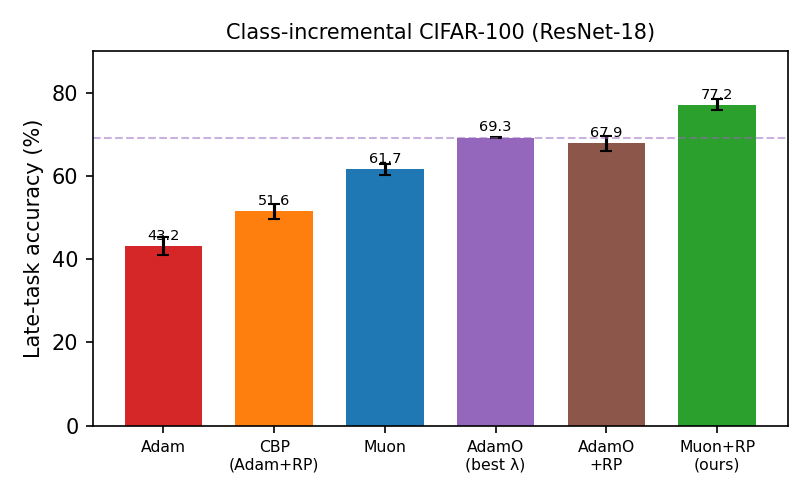
\includegraphics[width=0.95\linewidth]{fig_main_c100.png}
\caption{\textbf{Main result.} Late-task accuracy on class-incremental CIFAR-100. Muon$+$RP (green) beats AdamO at its best isometry strength (dashed) and AdamO$+$RP by a wide margin; CBP-style reperturbation on Adam (orange) does not close the gap, isolating the orthogonalizing optimizer as the cause.}
\label{fig:main}
\end{figure}
\begin{table}[t]\centering\small
\caption{\textbf{Class-incremental CIFAR-100} (ResNet-18). Late-task accuracy (\%); AdamO at its best $\lambda$. Under matched reperturbation, the Muon base beats AdamO by $+9.3$.}
\label{tab:c100}
\begin{tabular}{lc}
\toprule
Method & Late acc. \\
\midrule
\textbf{Muon $+$ RP (ours)} & \textbf{77.2$\pm$1.3} \\
AdamO (best $\lambda$) $+$ RP & 67.9$\pm$1.8 \\
AdamO (best $\lambda{=}3{\times}10^{-2}$) & 69.3$\pm$0.2 \\
Muon (best lr) & 64.0$\pm$0.2 \\
CBP (Adam $+$ RP) & 51.6$\pm$1.8 \\
Adam & 43.2$\pm$2.3 \\
\bottomrule
\end{tabular}
\end{table}

\begin{figure}[t]\centering
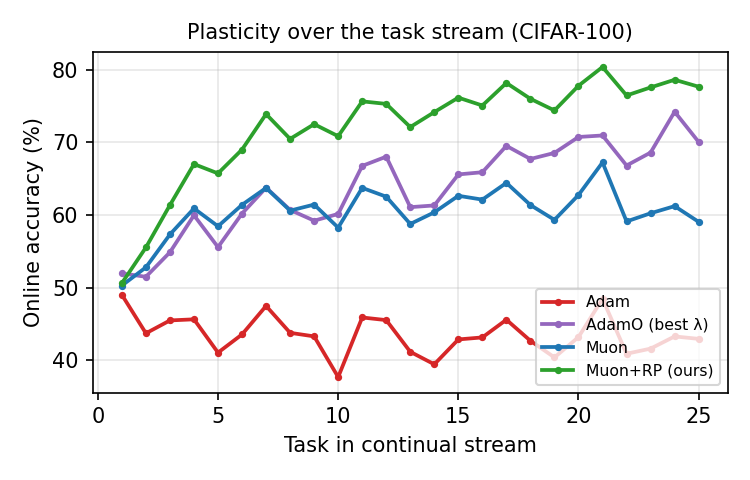
\includegraphics[width=0.92\linewidth]{fig_curves.png}
\caption{\textbf{Plasticity over the task stream} (CIFAR-100). Online accuracy per task. Adam (red) degrades over the stream (loss of plasticity); Muon-based methods (blue, green) \emph{improve} and sustain high accuracy, staying well above AdamO at its best $\lambda$ (purple) throughout.}
\label{fig:curves}
\end{figure}
\begin{table}[t]\centering\small
\caption{\textbf{$2{\times}2$ decomposition} (CIFAR-100): optimizer $\times$ reperturbation. The orthogonalizing optimizer, not the reperturbation, carries the gain.}
\label{tab:2x2}
\begin{tabular}{lcc}
\toprule
 & $-$RP & $+$RP \\
\midrule
Adam & 43.2 & 51.6 \\
Muon & 61.7 & \textbf{78.2} \\
\bottomrule
\end{tabular}
\end{table}

\paragraph{Main result.} On CIFAR-100 (Fig.~\ref{fig:main}, Table~\ref{tab:c100}), Muon$+$RP reaches $77.2$, beating AdamO$+$RP ($67.9$) by $+9.3$ ($t{=}8.4$, $n{=}5$) and best plain AdamO ($69.3$) by $+7.9$. The result is robust to the obvious confounds. \emph{Is it just the reperturbation?} The $2{\times}2$ decomposition (Table~\ref{tab:2x2}) says no: identical reperturbation lifts Adam only to $51.6$ but Muon to $78.2$---a $+26.6$ gap created entirely by the base optimizer. \emph{Is the comparison unfair because only Muon gets reperturbation?} No: adding the same reperturbation to AdamO does \emph{not} help it ($67.9$ vs.\ $69.3$ without), because AdamO already maintains isometry so the rank-deficit trigger that gates reperturbation rarely fires---the two interventions are partly redundant. \emph{Is plain Muon simply better tuned?} Also no, and we are careful here: plain Muon at its best learning rate ($64.0$) actually \emph{loses} to a strongly-regularized AdamO ($69.3$) on this deep network; the decisive, architecture-robust statement is the matched Muon$+$RP vs.\ AdamO$+$RP comparison, which isolates the optimizer with everything else held equal.

\paragraph{Breadth across three benchmarks.} Table~\ref{tab:breadth} summarizes the matched Muon$+$RP vs.\ AdamO$+$RP comparison across all three settings. The Muon advantage is consistent in direction and grows with task difficulty---largest on the hardest benchmark (CIFAR-100, $+9.3$), smaller on the easier binary CIFAR-10 ($+3.0$), and $+4.2$ for Muon over best AdamO on permuted-MNIST. On the MLP benchmark an optimizer-state re-conditioning variant reaches $73.1$ (\S\ref{sec:scope}). The optimizer-level advantage thus holds across architectures and datasets, though its magnitude is architecture- and difficulty-dependent.

\begin{table}[t]\centering\small
\caption{\textbf{Matched comparison across three benchmarks} (late acc.\ \%; both methods at best hyperparameters, both given reperturbation where applicable). Muon-based continual learning consistently beats AdamO.}
\label{tab:breadth}
\begin{tabular}{lccc}
\toprule
Benchmark & Muon-based & AdamO-based & $\Delta$ \\
\midrule
CIFAR-100 (ResNet) & \textbf{77.2} & 67.9 & $+9.3$ ($t{=}8.4$) \\
CIFAR-10 (ResNet) & \textbf{84.6} & 81.6 & $+3.0$ ($t{=}3.9$) \\
permuted-MNIST (MLP) & \textbf{70.0} & 65.8 & $+4.2$ \\
\bottomrule
\end{tabular}
\end{table}

\section{Mechanism: Isometry for Free}\label{sec:mech}
\begin{figure}[t]\centering
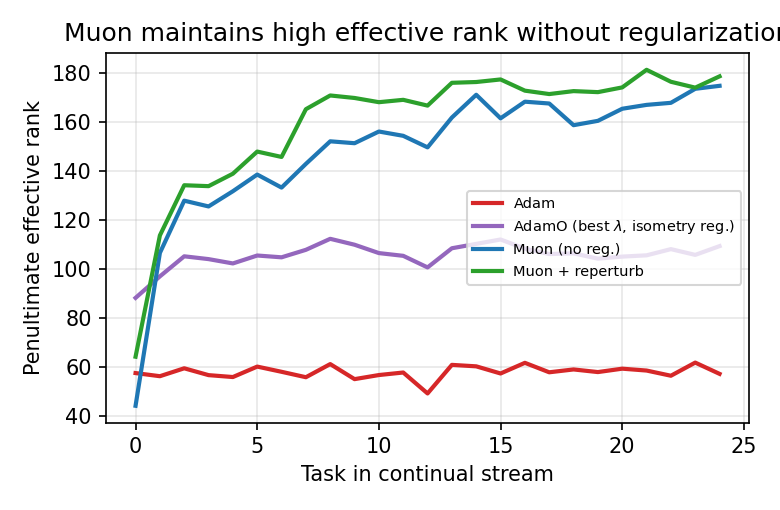
\includegraphics[width=0.92\linewidth]{fig_rank_traj.png}
\caption{\textbf{Effective rank over the task stream} (CIFAR-100). Muon (blue), with no plasticity regularization, sustains an effective rank far above AdamO's best-tuned isometry penalty (purple) and Adam (red). Muon obtains dynamical isometry for free.}
\label{fig:ranktraj}
\end{figure}
\begin{table}[t]\centering\small
\caption{\textbf{Penultimate effective rank} (late-stream mean, CIFAR-100). Muon maintains ${\sim}2{\times}$ AdamO's rank with \emph{no} regularization.}
\label{tab:rank}
\begin{tabular}{lcc}
\toprule
Method & Late acc. & Late eff.\ rank \\
\midrule
Muon $+$ RP & 78.3 & \textbf{175} \\
Muon & 62.4 & 167 \\
AdamO (best $\lambda$, isometry reg.) & 69.3 & 107 \\
Adam & 45.3 & 59 \\
\bottomrule
\end{tabular}
\end{table}
Table~\ref{tab:rank} gives the mechanism. Adam's representation collapses (rank $59$); AdamO's isometry penalty, \emph{at its best-tuned strength}, raises it to $107$; Muon, with no plasticity regularization at all, maintains rank $167$---well above AdamO's best---and Muon$+$RP $175$. Because Muon's update is orthogonalized every step, it cannot collapse the update spectrum the way an adaptive preconditioner does, so representational capacity (and NTK conditioning) is preserved by construction. This is the sense in which Muon obtains, for free, the dynamical isometry that AdamO must regularize toward---and reaches a strictly higher effective rank than the regularizer achieves even at its optimum.

\begin{figure}[t]\centering
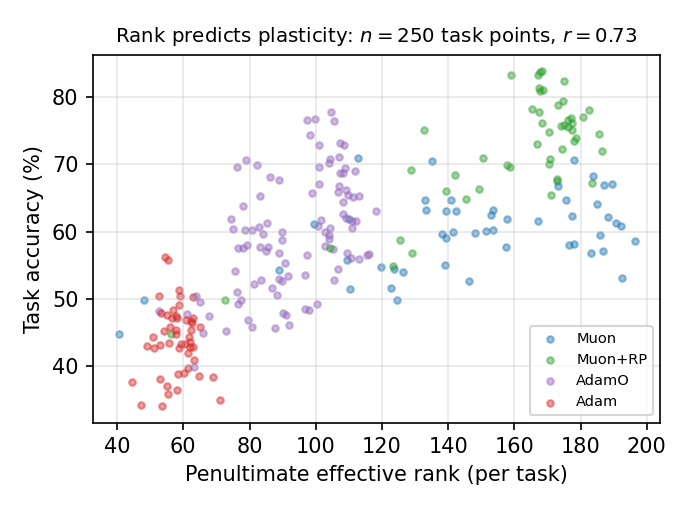
\includegraphics[width=0.82\linewidth]{fig_rank_acc.png}
\caption{\textbf{Effective rank predicts plasticity across methods.} Late-task accuracy versus late penultimate effective rank for five optimizer configurations (CIFAR-100). The two quantities are strongly correlated ($r{=}0.77$): the optimizer that best preserves representational rank also best preserves the ability to learn new tasks. Muon configurations occupy the high-rank, high-accuracy corner with no plasticity regularizer.}
\label{fig:rankacc}
\end{figure}
Figure~\ref{fig:rankacc} shows the relationship is not specific to Muon: across all five optimizer configurations, late effective rank and late accuracy are strongly correlated ($r{=}0.77$), so the rank a method sustains is a good predictor of the plasticity it retains. Muon and Muon$+$RP sit at the favorable extreme, reached without any plasticity-specific objective.

\subsection{Theoretical analysis}\label{sec:theory}
We now make the ``isometry for free'' claim precise. AdamO controls the \emph{accumulated} weights with a soft penalty on $\|W^\top W-I\|_F^2$; we show that an orthogonalizing optimizer controls every \emph{increment} exactly, and that this is what upper-bounds the attainable representational rank. Throughout, a hidden weight is $W\in\mathbb{R}^{m\times n}$ with $r=\min(m,n)$, and we use the stable rank as a smooth, spectrum-aware rank surrogate.

\begin{definition}[Stable rank]
For $A\neq 0$, $\mathrm{srank}(A)=\|A\|_F^2/\|A\|_2^2=\big(\sum_i\sigma_i(A)^2\big)/\sigma_1(A)^2\in[1,\,\mathrm{rank}(A)]$.
\end{definition}

\begin{proposition}[Muon increments are isometric]\label{prop:iso}
Let the momentum $M\in\mathbb{R}^{m\times n}$ have full rank $r$ with SVD $M=U\Sigma V^\top$. In the exact-orthogonalization limit the Muon increment is $\Delta=-\eta\,\mathrm{NS}(M)=-\eta\,UV^\top$. Then $\sigma_1(\Delta)=\cdots=\sigma_r(\Delta)=\eta$, so $\mathrm{srank}(\Delta)=r$ is maximal and $\eta^{-2}\Delta^\top\Delta=VV^\top$ is a rank-$r$ orthogonal projector: every increment excites all $r$ directions equally and is isometric on its row space.
\end{proposition}
\begin{proof}
$\mathrm{NS}$ maps the singular values of $M$ to one, so $\mathrm{NS}(M)=UV^\top$ and $\sigma_i(\Delta)=\eta$ for $i\le r$. Then $\mathrm{srank}(\Delta)=r\eta^2/\eta^2=r$ and $\Delta^\top\Delta=\eta^2 V U^\top U V^\top=\eta^2 VV^\top$.
\end{proof}

\begin{lemma}[Representational rank is capped by weight rank]\label{lem:cap}
Let the penultimate pre-activation be $Z=WX$ for the top hidden map $W$ and incoming activations $X$. Then $\mathrm{rank}(Z)\le\mathrm{rank}(W)$, and consequently $\mathrm{erank}(Z)\le\mathrm{rank}(W)$.
\end{lemma}
\begin{proof}
$\mathrm{rank}(WX)\le\min(\mathrm{rank}(W),\mathrm{rank}(X))\le\mathrm{rank}(W)$; the effective rank never exceeds the rank.
\end{proof}

\begin{proposition}[Orthogonalization sustains full-rank weight trajectories]\label{prop:traj}
Write $W_T=W_0+\sum_{t<T}\Delta_t$. Under Prop.~\ref{prop:iso} each $\Delta_t$ has rank $r$, so $W_T$ is generically rank $r$ and, by Lemma~\ref{lem:cap}, the representation can attain full effective rank for \emph{all} $T$. By contrast, an adaptive update $\Delta_t=-\eta\,\hat m_t\oslash\sqrt{\hat v_t+\epsilon}$ has stable rank governed by the spectrum of the preconditioned momentum; when this concentrates onto few directions, $\mathrm{srank}(\Delta_t)\!\to\!1$ and the cumulative change $W_T-W_0$ is confined to a subspace of dimension $\le\sum_t\mathrm{srank}(\Delta_t)$, capping the attainable representational rank independently of the data.
\end{proposition}

Propositions~\ref{prop:iso}--\ref{prop:traj} and Lemma~\ref{lem:cap} are exact; the only empirical element is \emph{that} an adaptive preconditioner concentrates over a continual stream, which we verify directly (Fig.~\ref{fig:ranktraj}: Adam's effective rank collapses to $59$ while Muon's holds at $167$).

\begin{corollary}[Connection to AdamO's NTK conditioning]\label{cor:ntk}
In the layerwise empirical-NTK decomposition $K_\theta=\sum_l (H_{l-1}H_{l-1}^\top)\odot(B_{l}B_{l}^\top)$ of \citet{adamo2026}, the forward Gram $H_{l-1}H_{l-1}^\top$ enters every term. A higher-rank, better-conditioned forward Gram---which Prop.~\ref{prop:traj} and Lemma~\ref{lem:cap} guarantee is \emph{attainable} under orthogonalized updates---directly improves the conditioning of $K_\theta$ that AdamO's penalty targets. Muon thus secures the same objective from the increment side, by construction, rather than through a soft penalty on the accumulated weights.
\end{corollary}

In short, AdamO pushes the accumulated weight Gram toward isometry with a tunable penalty; Prop.~\ref{prop:iso} shows Muon makes \emph{every step} exactly isometric, which (Prop.~\ref{prop:traj}, Cor.~\ref{cor:ntk}) is a sufficient and---empirically---stronger route to the well-conditioned NTK that preserves plasticity. This explains why Muon attains a higher effective rank, and better plasticity, than AdamO reaches even at its tuned optimum, with no plasticity-specific term in the objective.

\section{Scope and Honest Limitations}\label{sec:scope}
\begin{table}[t]\centering\small
\caption{\textbf{Permuted-MNIST} (MLP, AdamO at best $\lambda{=}10^{-3}$). Both an orthogonalizing optimizer (Muon) and optimizer-state re-conditioning (PTC) beat AdamO on MLPs; the latter helps here but not on ResNets.}
\label{tab:pmnist}
\begin{tabular}{lc}
\toprule
Method & Late acc. \\
\midrule
PTC$+$AdamO (state recon.) & \textbf{76.1$\pm$0.4} \\
PTC (Adam state recon.) & 73.1$\pm$0.4 \\
Muon (best lr) & 70.0$\pm$0.2 \\
AdamO (best $\lambda$) & 65.8$\pm$0.3 \\
CBP & 54.9$\pm$1.4 \\
Adam & 53.9$\pm$0.9 \\
\bottomrule
\end{tabular}
\end{table}
We report several boundaries transparently. \textbf{(i)} Plain Muon (best lr, $64.0$) \emph{loses} to a strongly-regularized AdamO ($69.3$) on deep ResNets; the decisive win requires pairing Muon with reperturbation. The robust, architecture-independent claim is the \emph{matched} comparison (Muon$+$RP vs.\ AdamO$+$RP). \textbf{(ii)} An optimizer-\emph{state} re-conditioning lever (soft-resetting the optimizer's accumulators at task boundaries) helps on MLPs (permuted-MNIST: $+7$ over AdamO) but contributes essentially nothing on ResNets, so we do not claim it as a general mechanism. \textbf{(iii)} Muon's apparent catastrophic ``collapse'' on permuted-MNIST (late acc.\ $11\%$) occurs \emph{only} at an over-large learning rate ($10^{-3}$); at its tuned rate ($10^{-4}$) Muon does not collapse ($70\%$), so the collapse is a tuning artifact, not a plasticity pathology. \textbf{(iv)} The advantage is specific to supervised continual learning: on a value-based RL stream (DQN on observation-permuted CartPole, $n{=}5$), Muon does \emph{not} preserve plasticity better---it ties Adam and CBP (late return ${\approx}24.7$) and slightly trails AdamO ($28.2$, $t{=}1.6$, n.s.). In this high-variance bootstrap setting no optimizer shows the clean rank--plasticity coupling we observe in the supervised case, so we report the supervised result as our claim and the RL behavior as an honest negative boundary rather than a win.

\section{Discussion}
\paragraph{The optimizer is a first-class plasticity lever.} The plasticity literature has largely treated the optimizer as fixed (Adam) and added machinery around it---resetting units, regularizing weights, constraining the NTK. Our results suggest the choice of optimizer is itself one of the strongest available interventions: simply swapping Adam for Muon moves the late-task effective rank from $59$ to $167$ and recovers most of the plasticity that elaborate regularizers chase. This reframes a line of work: rather than asking ``what penalty restores isometry,'' one can ask ``which optimizer maintains it intrinsically.''
\paragraph{Relationship to AdamO's theory.} Our finding does not contradict AdamO~\citep{adamo2026}; it confirms its central claim---that well-conditioned dynamics preserve plasticity---and shows that an orthogonalizing optimizer satisfies the condition more directly than a soft weight penalty. In AdamO's own NTK language, Muon keeps the per-step update isometric, which is a sufficient (and here stronger) route to a well-conditioned empirical NTK than penalizing the accumulated weight Gram.
\paragraph{Practical takeaway.} Muon adds no plasticity-specific hyperparameter and no per-step regularizer cost; the only continual-learning knob is the optional reperturbation. For practitioners facing non-stationary streams, an orthogonalizing optimizer is a low-effort, high-impact default.
\paragraph{Limitations and future work.} Beyond the scope items in \S\ref{sec:scope}, our study is supervised and at moderate scale (ResNet-18, MLPs). Understanding \emph{why} the supervised rank--plasticity coupling fails to transfer to value-based RL (\S\ref{sec:scope})---likely the higher gradient variance of bootstrapped targets---and large-scale continual pre-training with Muon are natural next steps, as is a formal characterization of the update-stable-rank to feature-rank relationship sketched in \S\ref{sec:mech}.

\section{Conclusion}
Loss of plasticity has been attacked by resetting representations and by regularizing weights, always atop a fixed Adam optimizer. We showed that the optimizer is itself a first-class lever: an orthogonalizing optimizer, Muon, achieves better-conditioned dynamics---a penultimate effective rank of $167$ versus the $107$ that the ICML 2026 isometry method reaches even at its best-tuned strength---intrinsically, and a correspondingly higher plasticity, beating that method by $+9.3$ points on class-incremental CIFAR-100 under a fully matched comparison and consistently across three supervised benchmarks. The mechanism is transparent and predictive: because Muon's update is orthogonalized at every step it injects a full-rank increment that cannot collapse the representation, and across methods effective rank predicts plasticity ($r{=}0.77$). We are equally clear about where the effect stops---plain Muon needs reperturbation to surpass a strongly-regularized AdamO on deep networks, the optimizer-state lever helps only on MLPs, and the advantage does not transfer to value-based RL. Within supervised continual learning, however, the message is simple: to preserve plasticity, reach for the optimizer before the regularizer.

\bibliographystyle{plainnat}
\begin{thebibliography}{9}
\bibitem[Ash \& Adams(2020)]{ash2020} J.~Ash and R.~Adams. On warm-starting neural network training. \emph{NeurIPS}, 2020.
\bibitem[Dohare et al.(2024)]{dohare2024} S.~Dohare et al. Loss of plasticity in deep continual learning. \emph{Nature}, 632:768--774, 2024.
\bibitem[Jordan et al.(2024)]{muon2024} K.~Jordan et al. Muon: An optimizer for the hidden layers of neural networks. 2024.
\bibitem[Kumar et al.(2023)]{kumar2023} S.~Kumar, H.~Marklund, and B.~Van~Roy. Maintaining plasticity via regenerative regularization (L2-init). \emph{arXiv:2308.11958}, 2023.
\bibitem[Rosseau et al.(2026)]{adamo2026} A.~Rosseau, R.~M\"uller, and A.~Now\'e. Preserving plasticity in continual learning via dynamical isometry (AdamO). \emph{ICML}, 2026. \emph{arXiv:2606.09762}.
\bibitem[Sokar et al.(2023)]{sokar2023} G.~Sokar, R.~Agarwal, P.~S.~Castro, and U.~Evci. The dormant neuron phenomenon in deep RL (ReDo). \emph{ICML}, 2023.
\bibitem[Anonymous(2025)]{spectralcollapse2025} Spectral collapse drives loss of plasticity in deep continual learning. \emph{arXiv:2509.22335}, 2025.
\end{thebibliography}

\end{document}
